\subsection{Status duration distribution modeling}
\label{section_lasting_time_modeling}
Similar to the modeling process of speed, we explore the cumulative distribution of lasting time. Then we fit the cumulative distribution to get the cumulative distribution formular and its estimated parameters.
The fit formulas are given as formulae \ref{formular_ccdf_lasting_time}, and the fitting results are shown as  fig. \ref{figure_fit_ccdf_lasting_time}.
\begin{equation}\label{formular_ccdf_lasting_time}
\begin{array}{ll}
 \phi(x)=1-exp(-e*x)& x\in [0,43200]\\
\end{array}
\end{equation}

\begin{figure}[htbp]
\centering
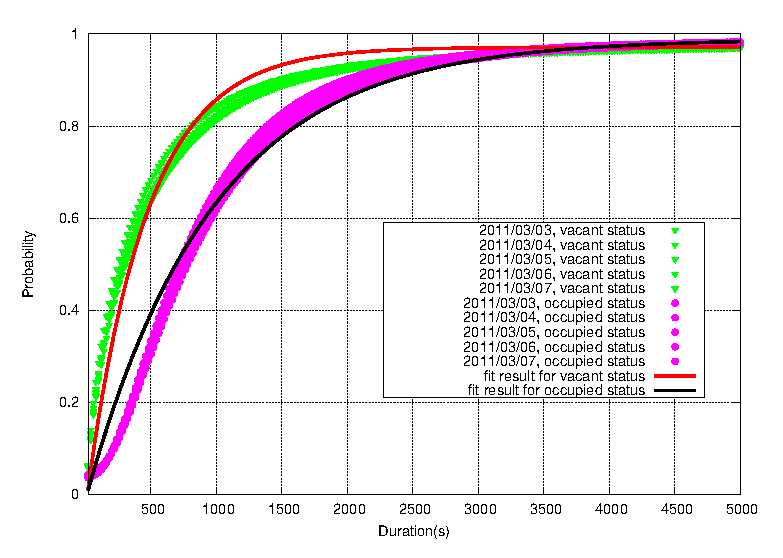
\includegraphics[width=0.4\textwidth]{figures/fit/duration_fit.eps}\\
\caption{The fit result of the cumulative status duration distributions.}\label{figure_fit_ccdf_lasting_time}
\end{figure}


The fitting result for status 0 is $\phi(x)_0=1-exp(-0.00149701*x)$, and the rms of residuals is 0.0347105. The fitting result for status 1 is $\phi(x)_1=1-exp(-0.000969622 *x)$  and the rms of residuals is 0.0337265.
